\section{Microcontroller}
\mult{2}

\begin{remark}
    \begin{itemize}
        \item Microcontroller
        \item System Bus
        \item Digital Logic Basics
        \item Synchronous Bus
        \item Control and Status Registers
        \item Address Decoding
        \item Slow Slaves (Peripherals)
        \item Bus Hierarchies
        \item Accessing Control Registers in C
        \item Conclusions
    \end{itemize} 
\end{remark}

\begin{theorem}{Embedded Systems}
    \begin{itemize}
        \item low cost (usb sticks, consumer electronics)
        \item low power (sensor networks, mobile devices)
        \item small size (smart cards, wearables)
        \item real time (anti-lock brakes, process control)
        \item reliability (medical devices, automotive)
        \item extreme environment (space, automotive)
    \end{itemize}
\end{theorem}

\begin{concept}{Single Chip Solution} \\
    $\Rightarrow$ CPU with integrated memory and peripherals
\end{concept}

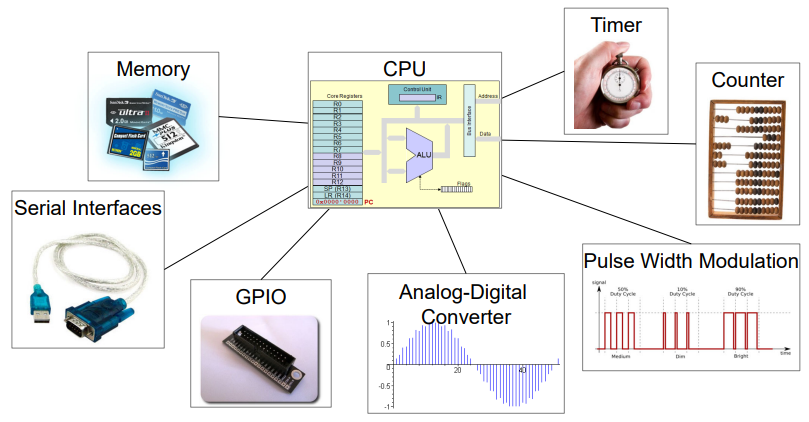
\includegraphics[width=\linewidth]{single_chip_solution.png}

\multend

\subsection{Microcontroller Architecture}

\subsubsection{Peripherals and Registers}


\begin{definition}{Peripherals}

    \begin{minipage}{0.35\linewidth}
    \begin{itemize}
        \item configurable hardware blocks \\ of a microcontroller
        \item accepts specific task from CPU, \\ executes task and returns result \\ (status, e.g. task completion, error)
        \item often interfaces to outside world\\
        many (not all) interact with \\ external MCU pins 
        \item examples: GPIO, UART, SPI, ADC
    \end{itemize}
    \end{minipage}
    \begin{minipage}{0.64\linewidth}
        \vspace{-5mm}
        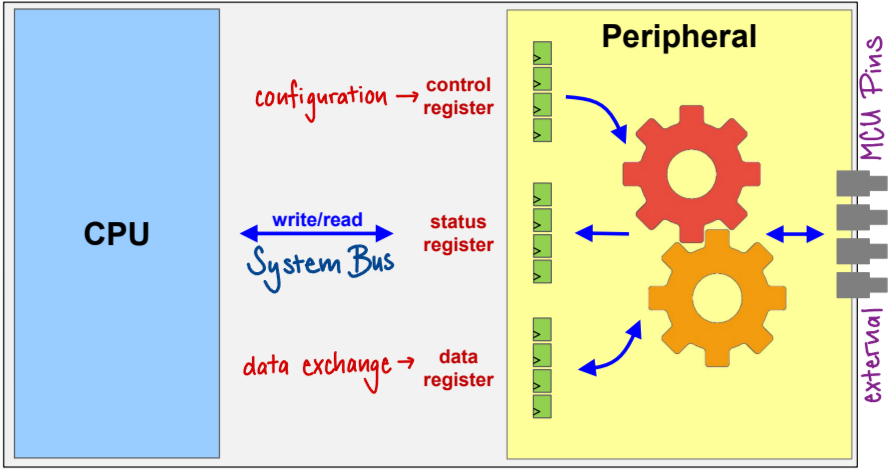
\includegraphics[width=\linewidth]{peripherals_registers.png}
    \end{minipage}
\end{definition}

\mult{2}

\begin{concept}{Peripheral Registers}
    CPU controls/monitors Peripherals through registers:
    \begin{itemize}
        \item Registers are arrays of flip-flops (storage elements with two states, i.e. 0 or 1)
        \item Each flip-flop stores one bit of information
        \item CPU writes to and reads from registers
    \end{itemize}
\end{concept}

\begin{theorem}{Categories of Registers}
    \begin{itemize}
        \item \textbf{Control Registers} \\
        enable CPU to configure the peripheral
        \item \textbf{Status Registers} \\
        enable CPU to monitor the peripheral
        \item \textbf{Data Registers} \\
        enable CPU to exchange data with the peripheral
    \end{itemize}
\end{theorem}

\begin{examplecode}{Memory-mapped Peripheral Registers}\\
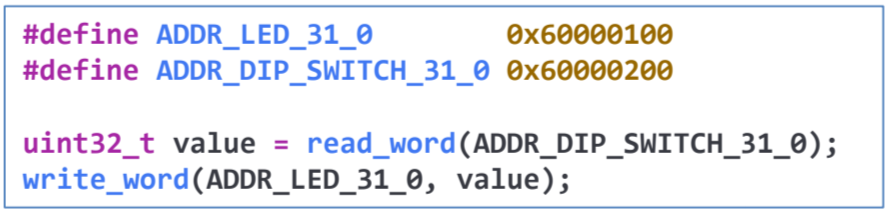
\includegraphics[width=\linewidth]{led_dip_switches_peripherals_examples.png}
\end{examplecode}

\begin{definition}{Memory-mapped Peripheral Registers}
    \begin{itemize}
        \item Control register: controls states of LEDs
        \item Status register: monitors states of DIP switches
    \end{itemize}
    \vspace{1mm}
    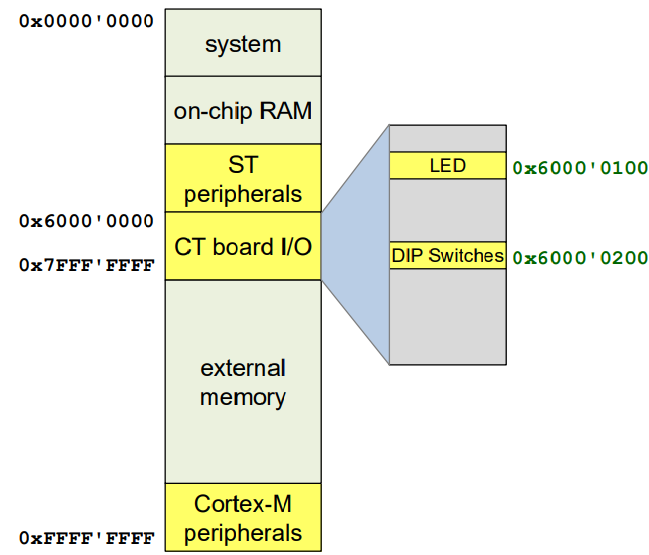
\includegraphics[width=\linewidth]{registers_leds_dipswitches.png}
\end{definition}

\multend

\begin{concept}{CPU access to individual Peripheral Registers}
    \begin{itemize}
        \item ARM \& STM map the peripheral registers into
        the memory address range
        \item Reference Manual shows the defined addresses
    \end{itemize}
    \vspace{2mm}
    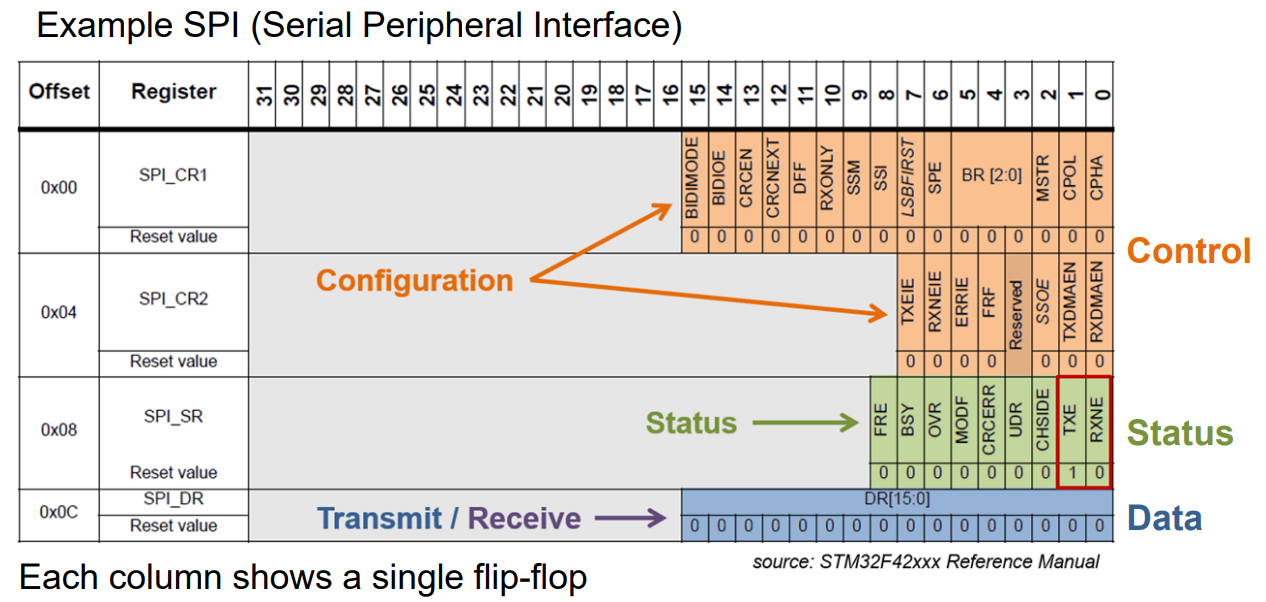
\includegraphics[width=\linewidth]{example_SPI_cpu_access.png}
\end{concept}

\mult{2}

\begin{definition}{Memory mapping of Peripheral Registers}
    \begin{itemize}
        \item Each peripheral register has a unique address
        \item CPU uses the address to access the register
        \item CPU uses load/store instructions to access the register
    \end{itemize}
    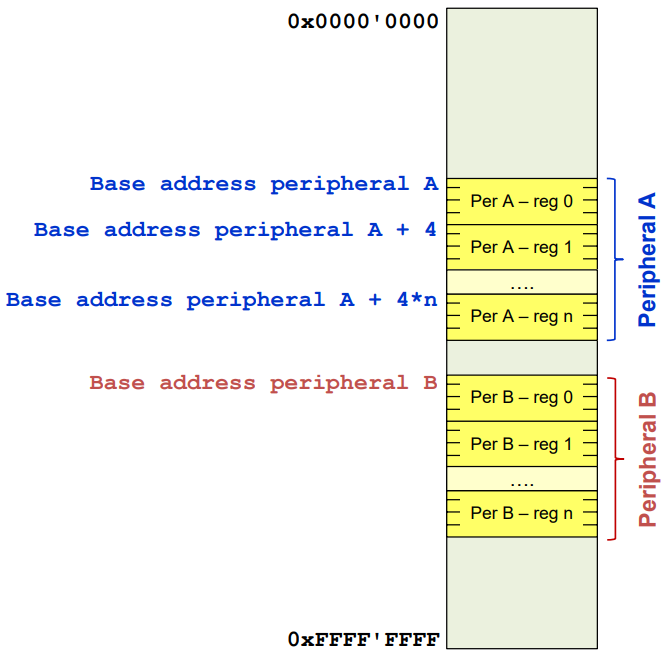
\includegraphics[width=\linewidth]{peripheral_registers_cpu_access.png}
\end{definition}

\begin{concept}{CPU read/write to peripheral registers}\\
    How does the CPU write to and read from peripheral registers?
    \vspace{-2mm}\\
    \begin{itemize}
        \item CPU reads/writes to peripheral registers
        \item CPU uses memory-mapped I/O to access peripheral registers
        \item CPU uses load/store instructions to access peripheral registers
    \end{itemize}
    $\Rightarrow$ System Buses
\end{concept}

\multend


\subsubsection{System Bus}
\mult{2}

\begin{definition}{System Bus}
    \begin{itemize}
        \item Interconnects CPU with memory and peripherals
        \item CPU acts as master: initiating and controlling all transfers
        \item Peripherals and memory act as slaves: responding to requests from the CPU
        \item System bus is a shared resource
    \end{itemize}
    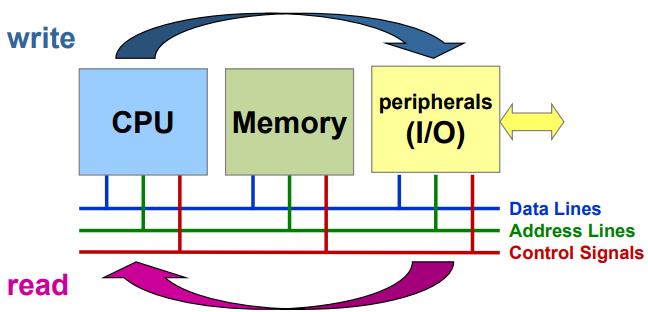
\includegraphics[width=\linewidth]{system_bus.png}
\end{definition}

\begin{concept}{Bus Specification}
    \begin{itemize}
        \item \textcolor{darkblue}{\textbf{Protocol and operations}}
        \item \textcolor{darkred}{\textbf{Signals}}
        \begin{itemize}
            \item Number of Signals
            \item Signal descriptions
        \end{itemize}
        \item \textcolor{darkgreen}{\textbf{Timing}}
        \begin{itemize}
            \item Frequency
            \item Setup and hold times
        \end{itemize}
        \item \textcolor{darkpurple}{\textbf{Electrical properties}} (not in exam)
        \begin{itemize}
            \item Drive strength and Load
        \end{itemize}
        \item \textcolor{darkorange}{\textbf{Mechanical requirements}} (not in exam)
    \end{itemize}
\end{concept}

\begin{theorem}{Signal Groups}
    \begin{itemize}
        \item \textcolor{darkblue}{\textbf{Data lines}}
        \begin{itemize}
            \item Bidirectional (read/write)
            \item Number of lines $\rightarrow$ data bus width \\(8, 16, 32, 64 parallel lines of data)
            \item Example: Cortex-M has 32 address lines $\rightarrow$ 4GB address space \\ $\rightarrow$ \texttt{0x00000000} to \texttt{0xFFFFFFFF}
        \end{itemize}
        \item \textcolor{darkgreen}{\textbf{Address lines}}
        \begin{itemize}
            \item Unidirectional: from Master to slaves
            \item Number of lines $\rightarrow$ size of address space
        \end{itemize}
        \item \textcolor{darkred}{\textbf{Control signals}}
        \begin{itemize}
            \item Control read/write direction
            \item Provide timing information
            \item Chip select, read/write, etc.
        \end{itemize}
    \end{itemize}
    \vspace{2mm}
    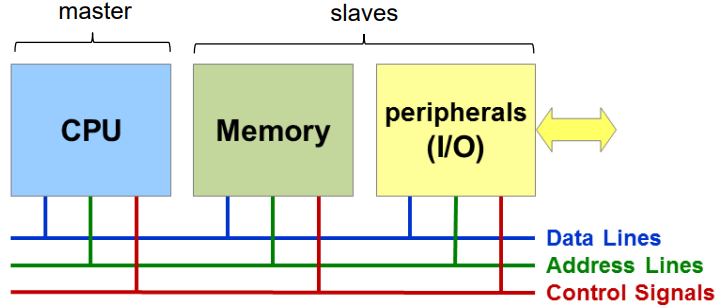
\includegraphics[width=\linewidth]{master_slave_signal_groups.png}
\end{theorem}

\multend

\begin{theorem}{Bus Timing Options}
    \vspace{2mm}\\
    \begin{minipage}{0.65\linewidth}
    \textbf{Synchronous}
    \begin{itemize}
        \item \textcolor{blue}{Master} and \textcolor{darkcorn}{slaves} use a common clock\\
        Often a dedicated clock signal from master to slave, \\ but clock can also be encoded in a data signal
        \item Clock edges control bus transfer on both sides
        \item Used by most on-chip buses
        \item Off-chip: DDR and synchronous RAM
    \end{itemize}
    \end{minipage}
    \begin{minipage}{0.2\linewidth}
        \vspace{-9mm}
        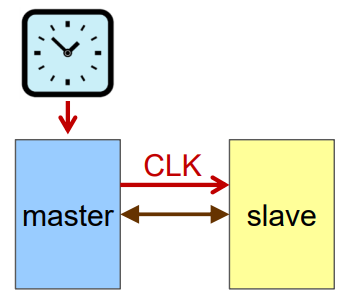
\includegraphics[width=\linewidth]{synchronous_bus_timing.png}
    \end{minipage}

    \begin{minipage}{0.65\linewidth}
    \textbf{Asynchronous}
    \begin{itemize}
        \item \textcolor{darkcorn}{Slaves} have no access to clock of the \textcolor{blue}{master}
        \\ $\rightarrow$ slave has their own clock or no clock at all
        \item Control signals carry timing information to allow synchronization
        \item Widely used for low data-rate off-chip memories \\
        $\rightarrow$ parallel flash memories and asynchronous RAM
    \end{itemize}
    \end{minipage}
    \begin{minipage}{0.2\linewidth}
        \vspace{-2mm}
        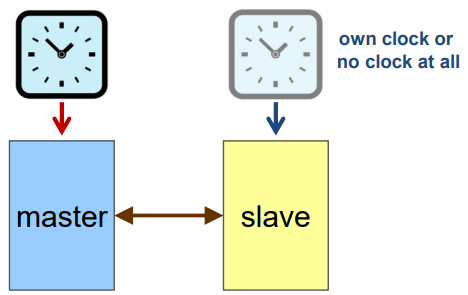
\includegraphics[width=\linewidth]{asynchronous_bus_timing.png}
    \end{minipage}
\end{theorem}

\mult{2}

\begin{corollary}{Multiple devices driving the same data line}\\
    What if one device drives a logic 1 (Vcc) and another device drives a logic 0 (Gnd)?\\
    $\Rightarrow$ Electrical short circuit!
    \\ $\rightarrow$ bus contention ('Streitigkeit')\\
    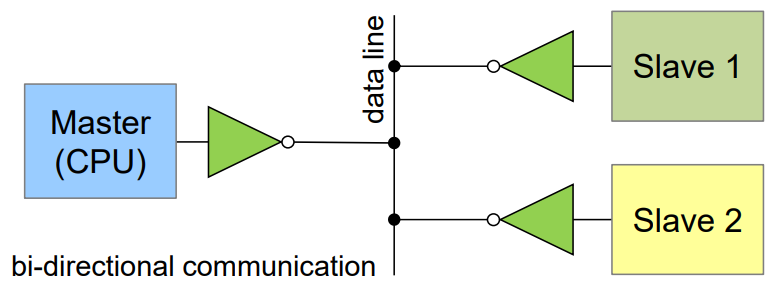
\includegraphics[width=\linewidth]{bus_contention.png}\\
    \small{Figure only shows output paths, input paths are not shown.}

\end{corollary}

\begin{concept}{Bus Contention} \\
    CPU defines who drives the data bus at which moment in time:
    \begin{itemize}
        \item \texttt{write} CPU drives bus $rightarrow$ all slave drivers disconnected
        \item \texttt{read} CPU releases bus $rightarrow$ one slave drives bus (selected through values on address lines, other slave drivers disconnected)
    \end{itemize}
    
    Electrically disconnecting a driver is called \textbf{tri-state} or \textbf{high-impedance} (Hi-Z) state. (switch)
    
    \important{CHECK IF CORRECT}
\end{concept}

\multend

\important{But how can a driver be disconnected electrically?}

\subsection{Digital Logic Basics}

\begin{definition}{CMOS Inverter}
    Complementary switches (transistors)\\
    $\rightarrow$ \textcolor{red}{p-type} and \textcolor{blue}{n-type} have opposite open-close behaviour\\
    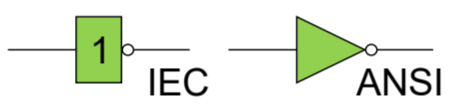
\includegraphics[width=0.3\linewidth]{cmos_inverter0.png}

    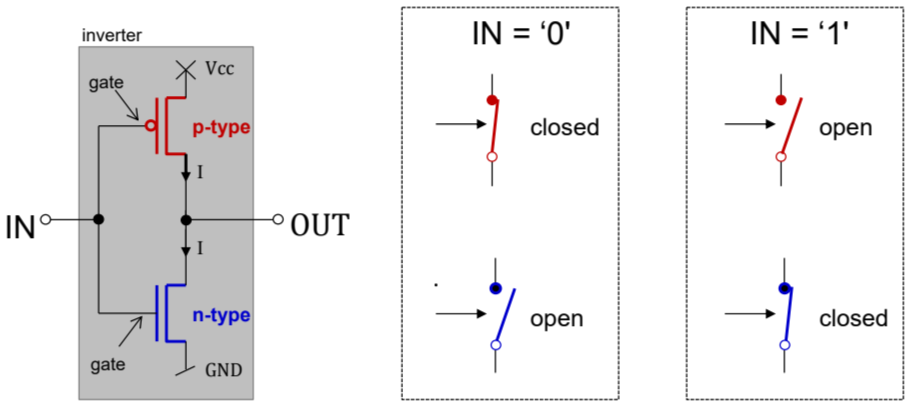
\includegraphics[width=\linewidth]{cmos_inverter1.png}\\
    e.g. Vcc = 3V = '1', Gnd = 0V = '0'\\
    Vcc is the supply voltage of the circuit/chip
    \vspace{2mm}\\
    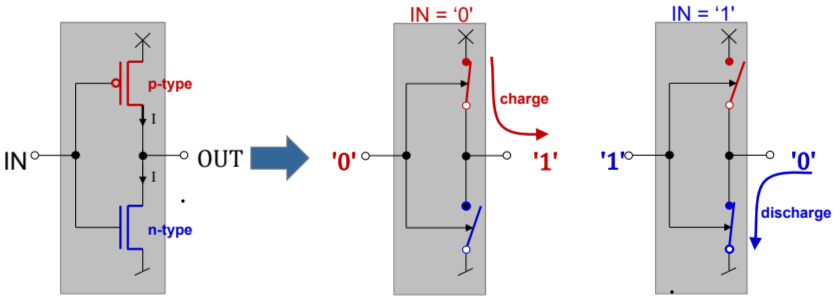
\includegraphics[width=\linewidth]{cmos_inverter2.png}\\
    A buffer is built by connecting two inverters in series
\end{definition}

\begin{definition}{CMOS Tri-State Inverter}\\
    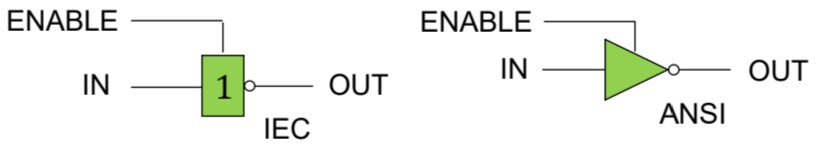
\includegraphics[width=\linewidth]{tristate_inverter1.png}\\
    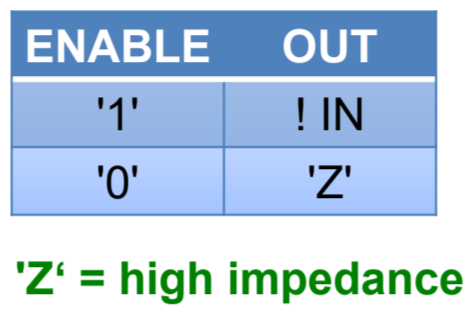
\includegraphics[width=\linewidth]{tristate_inverter2.png}\\
    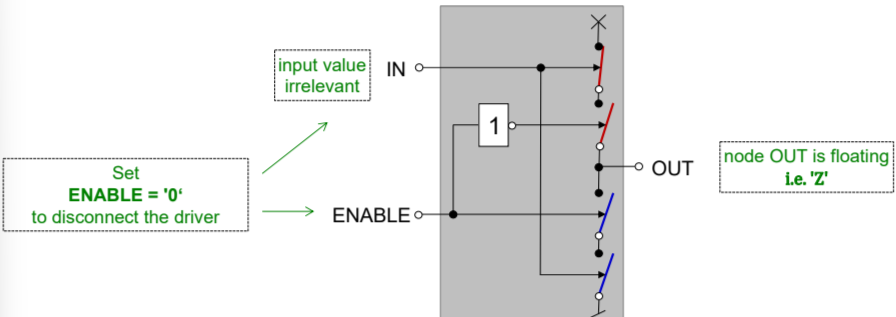
\includegraphics[width=\linewidth]{tristate_inverter3.png}\\
    Implementation:\\
    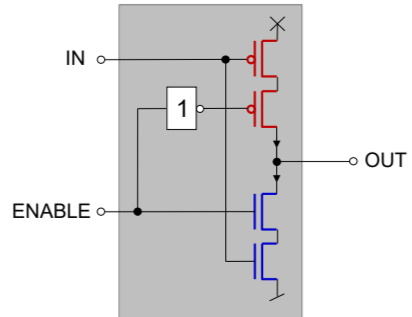
\includegraphics[width=\linewidth]{tristate_inverter4.png}
\end{definition}

\begin{concept}{Tri-State Buffer} Timing Diagram\\
    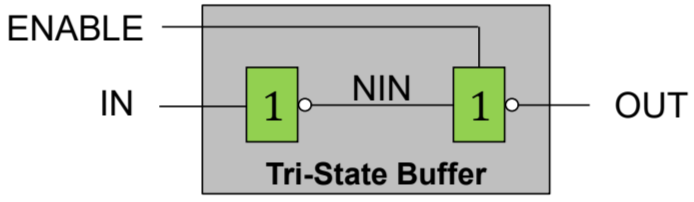
\includegraphics[width=\linewidth]{tristate_buffer1.png}\\
    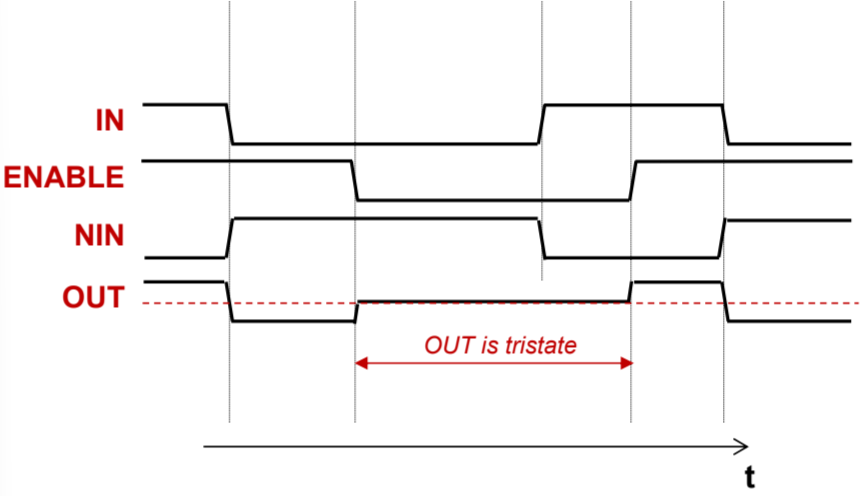
\includegraphics[width=\linewidth]{tristatebuffer2.png}\\
    When a signal like OUT is in tristate, we often say that it is 'floating'. 
    The term expresses that such a signal can easily be moved by parasitic electrical effects
    to either one of the reference levels, i.e. '0' or '1'.
\end{concept}

\begin{theorem}{Bus Timing Diagrams} Notation for Groups of Signals\\
    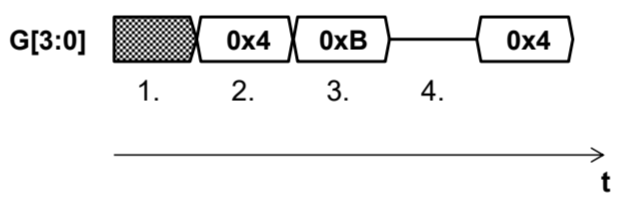
\includegraphics[width=\linewidth]{bus_timing_notation.png}\\
    Group G of 4 signals
1. unknown values

The values on each of the 4 signals are either ' 1 ' or ' 0 ', but unknown.
2. The bus holds the value $0 \times 4$

$$
\text { i.e. } \mathrm{G}[3]=\text { ' } 0 \text { ', G[2] = '1', G[1] = '0', G[0] = '0' }
$$

3. The bus holds the value $0 \times B$

$$
\text { i.e. } \mathrm{G}[3]=\text { ' } 1 \text { ', G[2] = '0', G[1] = '1', G[0] = '1' }
$$

4. Tri-state

All signals $\mathrm{G}[3: 0$ ] are tri-state (i.e. ' $Z$ ' or high-impedance). "No one is driving the bus"
\end{theorem}



\subsection{Synchronous Bus}

\begin{definition}{Synchronous Bus}\\
    Example Uses External Bus from ST Microelectronics
- Reason: Internal workings of the system bus are not disclosed by STM
- Signal names, bus protocol and timing based on external synchronous STM32F429xx mode instead
- For details see
- Chapter 37, Flexible memory controller (FMC) in ST Reference Manual RM0090
- Datasheet STM32F429xx

Figure 60 Synchronous non-multiplexed NOR/PSRAM read timings
Figure 61 Synchronous non-multiplexed PSRAM write timings
Naming Convention
- Letter ' N ' prefix in signal name ( $\mathrm{N} x x x$ ) means active-low signal
- E.g. NOE means 'NOT OUTPUT ENABLE'

NOE $=$ ' 0 ' $\rightarrow$ output enabled\\
NOE $=$ ' 1 ' $\rightarrow$ output disabled
\end{definition}

\begin{formula}{Block Diagram}

    \begin{minipage}{0.35\linewidth}
    \begin{itemize}
        \item Address lines [31:0]
        \item Data lines [31:0]
        \item Control signals
        \begin{itemize}
            \item CLK $\rightarrow$ clock
            \item NE $\rightarrow$ Not enable
            \item NWE $\rightarrow$ Not write enable
            \item NOE $\rightarrow$ Not output enable
        \end{itemize}
    \end{itemize}
    \end{minipage}
    \begin{minipage}{0.4\linewidth}
    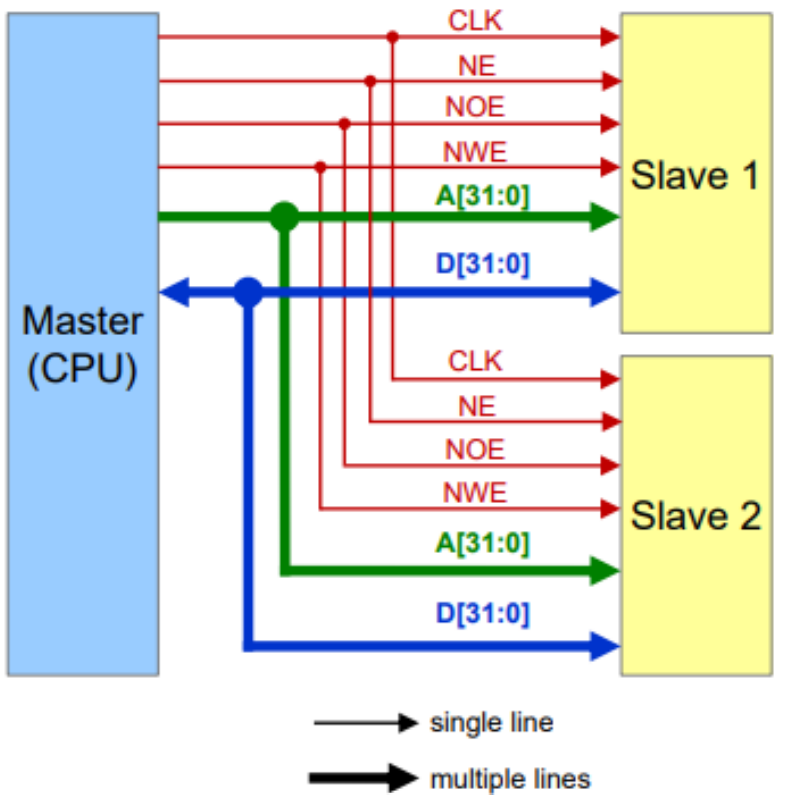
\includegraphics[width=\linewidth]{block_diagramm.png}
    \end{minipage}
\end{formula}

\begin{definition}{Bus Timing Diagram}
    \begin{itemize}
        \item CLK $\rightarrow$ clock signal (rising edge)
        \item NE $\rightarrow$ Not enable (active low)
        \item NWE $\rightarrow$ Not write enable (active low)
        \item NOE $\rightarrow$ Not output enable (active low)
    \end{itemize}
    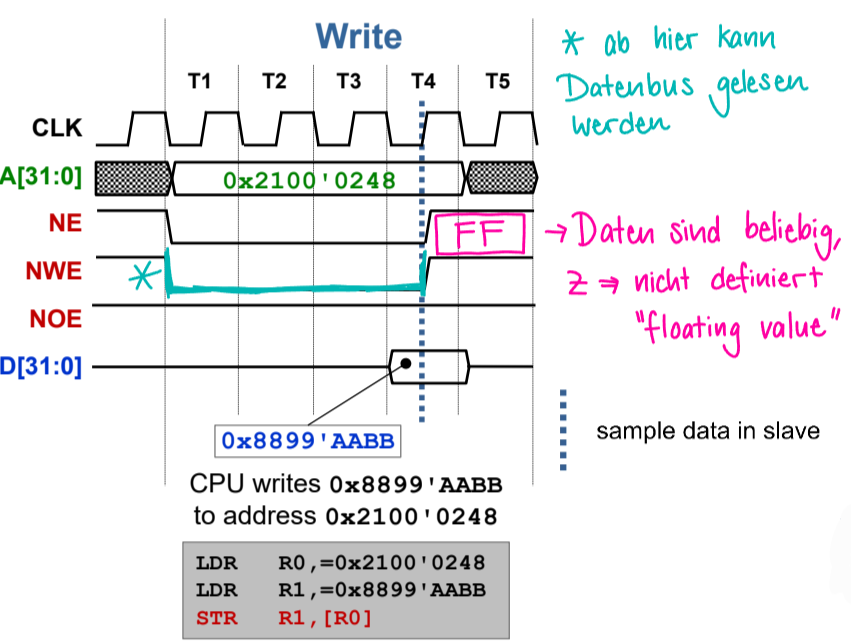
\includegraphics[width=\linewidth]{timing_diagram1.png}\\
    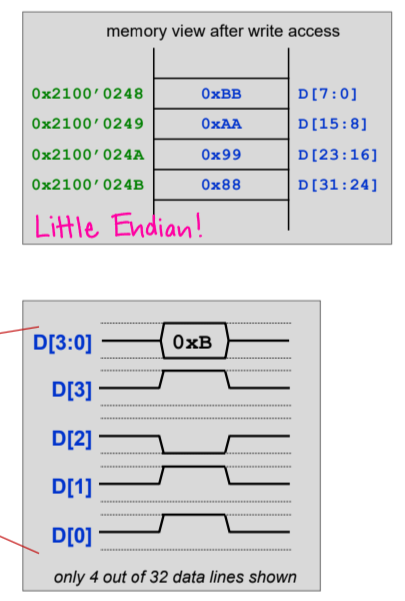
\includegraphics[width=\linewidth]{timing_diagram2.png}\\
    WICHTIG: nicht genau mit Flanke schreiben, Daten brauchen eine gewisse Zeit um stabil zu werden (keine genaue Definition, muss halt einfach 'genug' sein)\\
    READ dauert länger als WRITE, da die Daten erst stabil werden müssen bevor sie gelesen werden können\\
\end{definition}

\begin{formula}{Timing Diagram}  
    \begin{itemize}
        \item \texttt{write} \textcolor{darkblue}{D[:]} to \textcolor{darkgreen}{A[:]} $\rightarrow$ \textcolor{darkred}{NE, NWE} = 0
        \item \texttt{read} \textcolor{darkblue}{D[:]} from \textcolor{darkgreen}{A[:]} $\rightarrow$ \textcolor{darkred}{NE, NOE} = 0
    \end{itemize}
    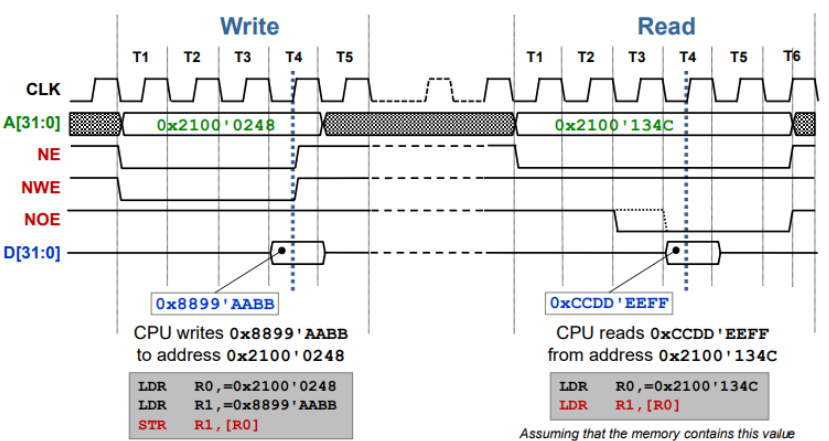
\includegraphics[width=\linewidth]{timing_diagram.png}
\end{formula}


\begin{theorem}{Bus Access Size}
    is determined by the NBL (0-3) (No Byte Line) signals
    \begin{itemize}
        \item NBL = 1 $\rightarrow$ Byte used for Read/Write
        \item NBL = 00
        \item NBL[0:3] = 0011 $\rightarrow$ Read Halfword
        \item NBL[0:3] = 1111 $\rightarrow$ Read Word
    \end{itemize}
    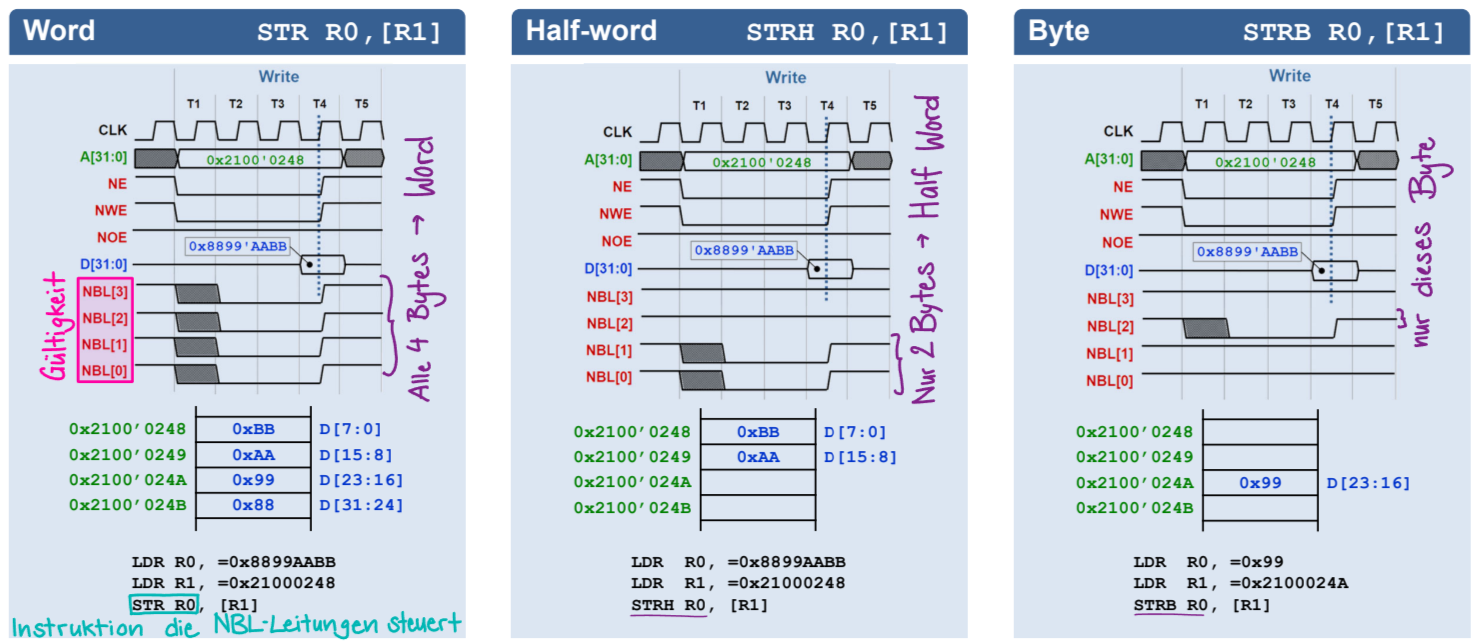
\includegraphics[width=\linewidth]{bus_access_size.png}\\
    Gültigkeit: damit zeigt die CPU an, welche der 4 Bytes übertragen werden sollen (gültig = 0 (unten))\\
    \begin{itemize}
        \item Exact Position of falling edge on NBL varies with chip version
        \item Value on unused data lines are unknown, figues show assumptions
    \end{itemize}
\end{theorem}




\subsubsection{Control and Status Registers}

\begin{definition}{Hardware Slave (Peripheral)}\\
    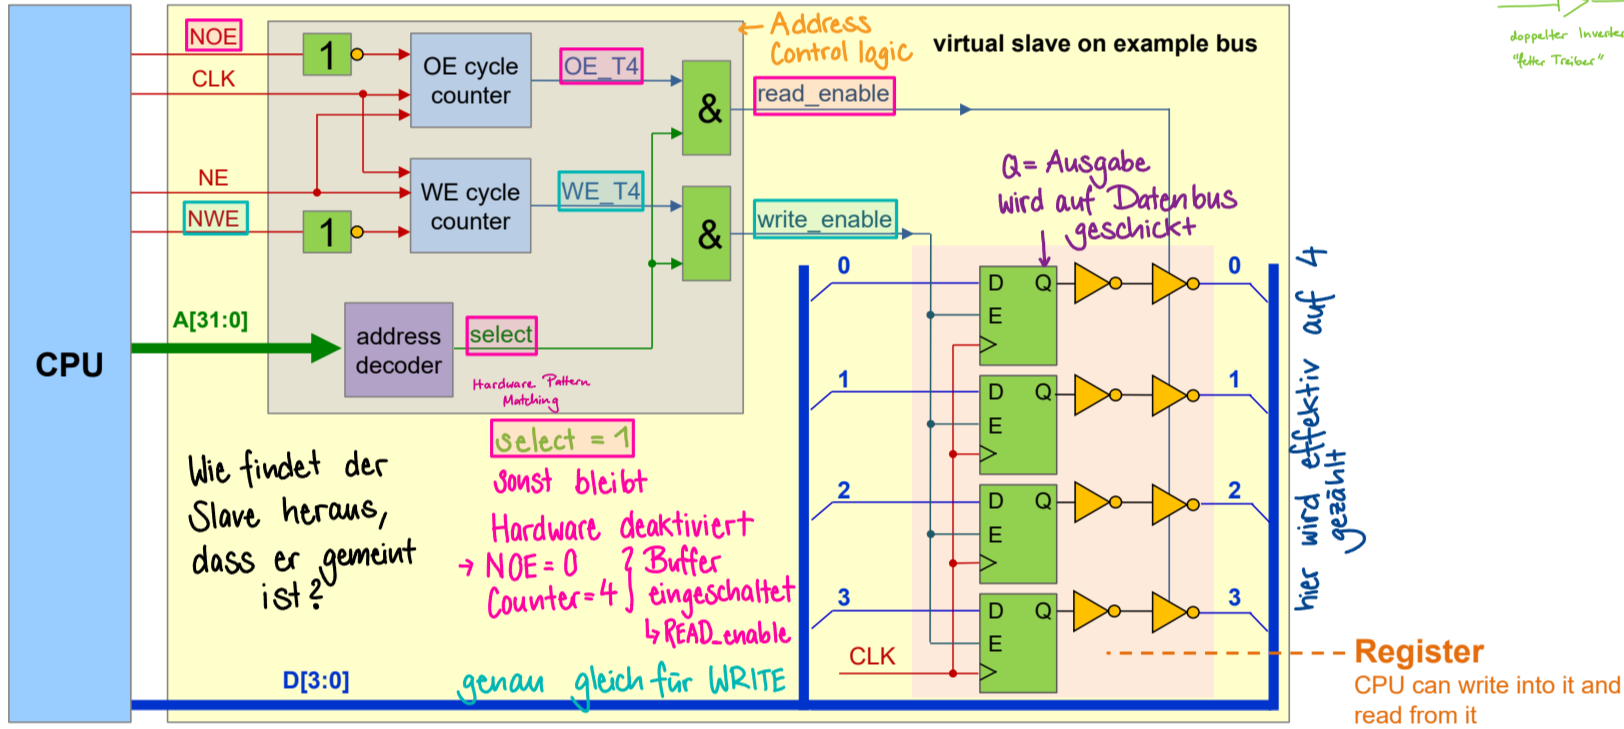
\includegraphics[width=\linewidth]{hardware_slave.png}
\end{definition}

\mult{2}

\begin{concept}{Control Bits}
    \begin{itemize}
        \item Allow CPU to configure Slaves
        \item CPU writes to register bit to configure Slave
        \item Slave uses output of register bit to configure itself
        \item Example: SPI Slave Select (SS) bit
        \item Usually read/write access to control bits
    \end{itemize}
\end{concept}

\begin{concept}{Status Bits}
    \begin{itemize}
        \item Allow CPU to monitor Slaves
        \item CPU reads register bit to monitor Slave
        \item Slave uses input of register bit to monitor itself (Slave writes to register bit)
        \item Example: SPI Busy bit
        \item Usually read-only access to status bits
    \end{itemize}
\end{concept}

\multend

\begin{example}
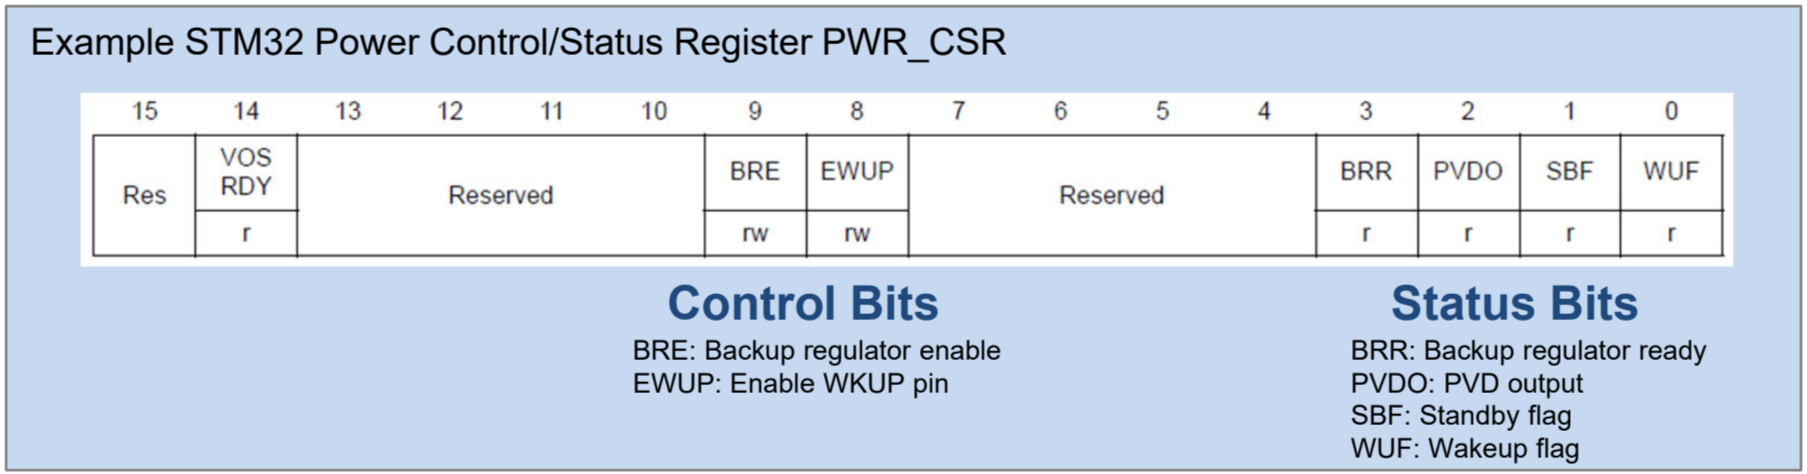
\includegraphics[width=\linewidth]{example_control_status_regs.png}\\
Control/Status register on example bus:\\
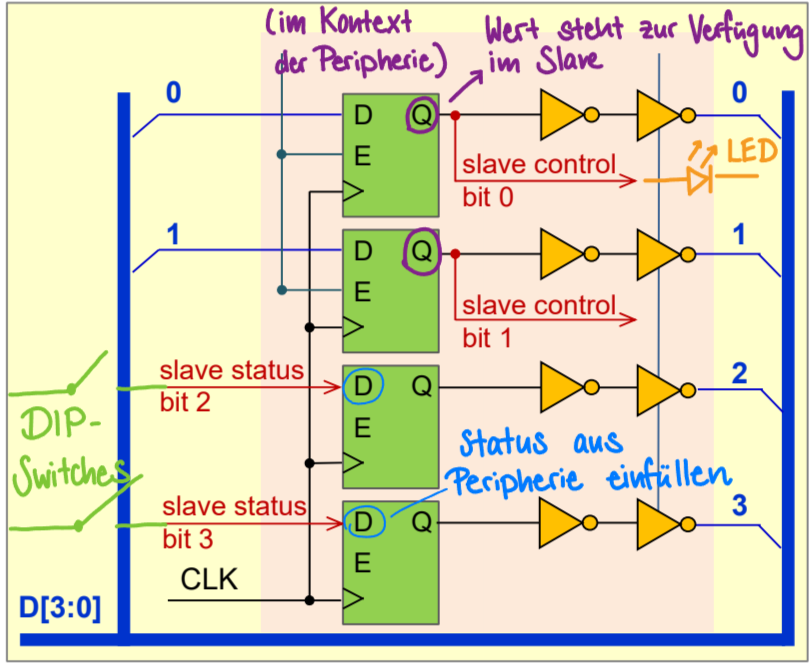
\includegraphics[width=\linewidth]{example_control_status_regs2.png}\\
control bits: 0 and 1\\
status bits: 2 and 3\\
The same register may contain both control and status bits!
\end{example}

\begin{theorem}{Control and Status Registers on CT Board}\\
    Chip-internal and external registers (details on memory map in STM32 Reference Manual)\\
    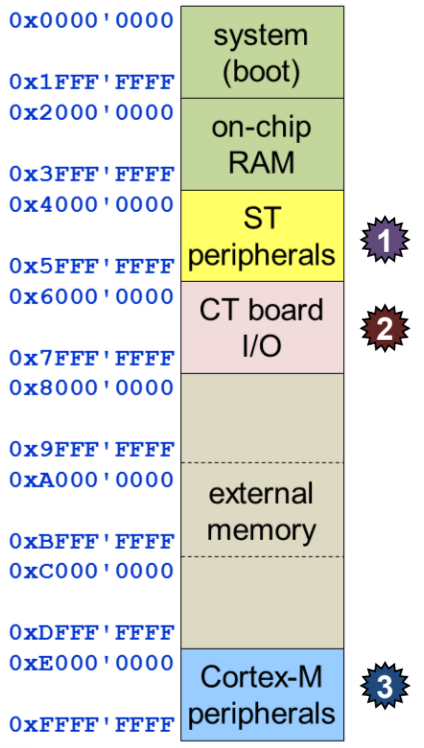
\includegraphics[width=\linewidth]{control_status_regs_ctboard1.png}\\
    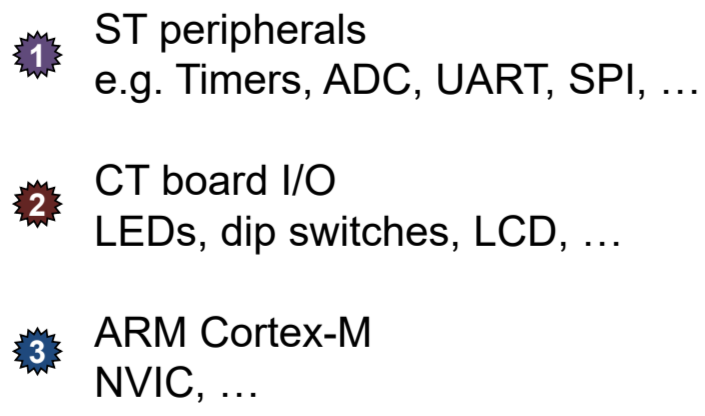
\includegraphics[width=\linewidth]{control_status_regs_ctboard2.png}\\
    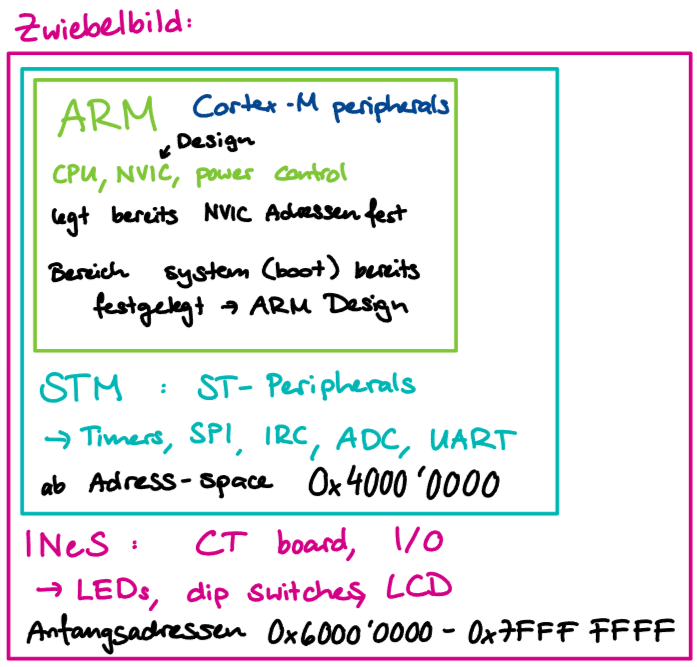
\includegraphics[width=\linewidth]{control_status_regs_ctboard3.png}
\end{theorem}

\subsubsection{Address Decoding}

\begin{remark}
    How does a Slave know that it is being addressed?\\
    $\Rightarrow$ Address decoding logic in the Slave (each on its own)
\end{remark}

\begin{definition}{Address Decoding}\\
    Interpretation of address line values. See whether bus access targets a particular address or address range.
    \begin{itemize}
        \item CPU uses address lines to select a peripheral
        \item Each peripheral has a unique address range
        \item Address decoding logic generates a chip select signal for each peripheral
    \end{itemize}

    \textbf{Full Address Decoding}
    \begin{itemize}
        \item All address lines are decoded
        \item A control register can be accessed at exactly one location
        \item 1:1 mapping: A unique address maps to a single hardware register
        \item example: LEDs and DIP switches on CT board
    \end{itemize}

    \textbf{Partial Address Decoding}
    \begin{itemize}
        \item Only a subset of address lines are decoded
        \item A control register can be accessed at multiple locations
        \item 1:n mapping: Multiple addresses map to the same hardware register
        \item Motivation: Simpler and possible Aliasing (Map a hardware register to several addresses)
    \end{itemize}
    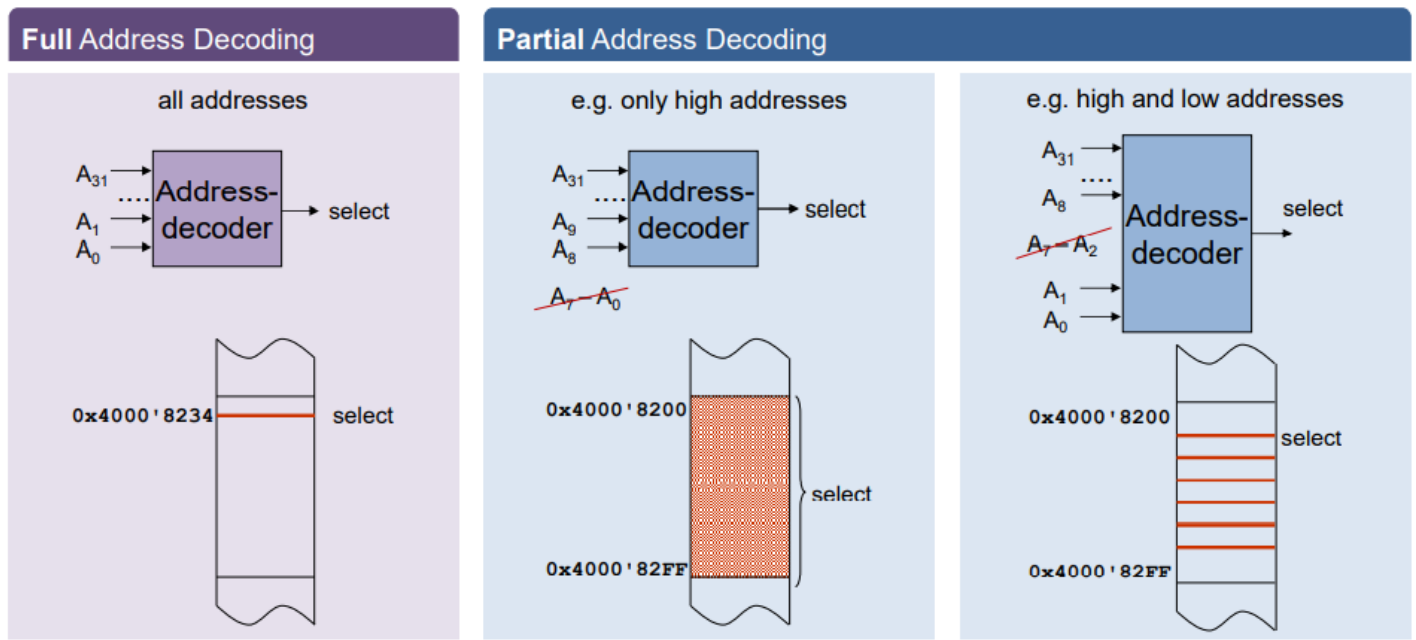
\includegraphics[width=\linewidth]{address_decoding.png}
\end{definition}

\begin{example}
    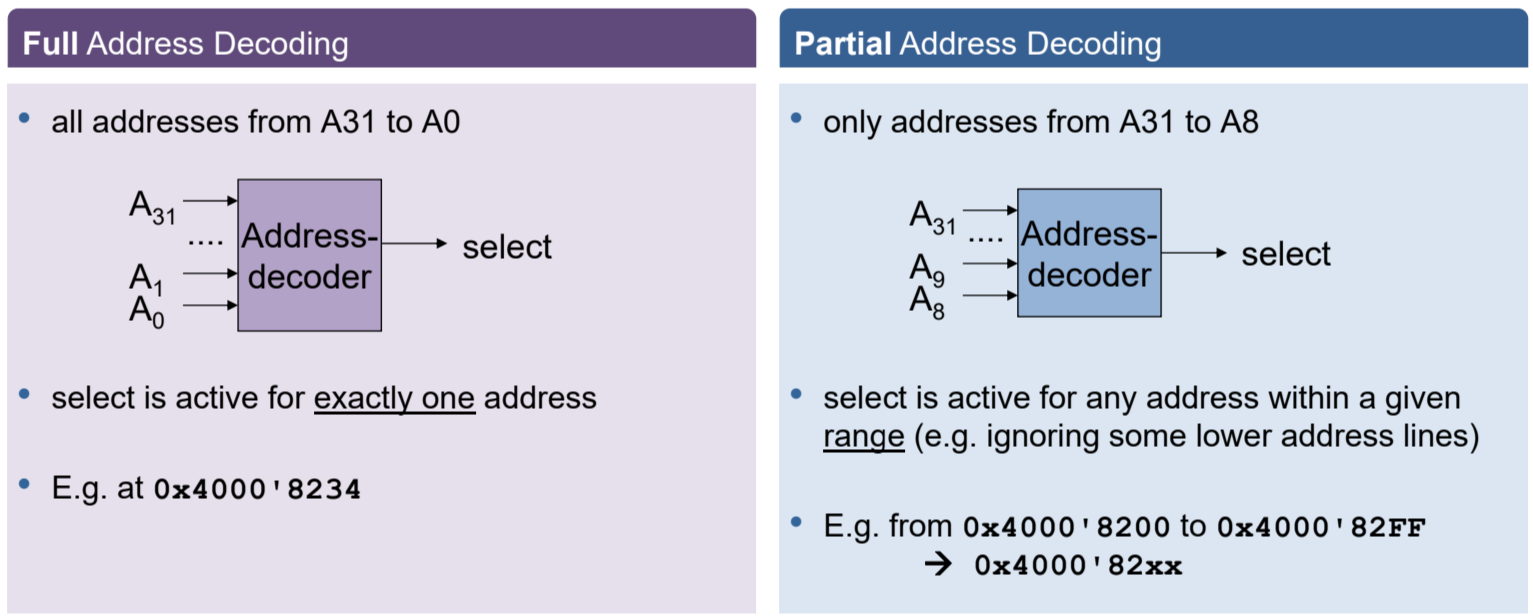
\includegraphics[width=\linewidth]{example_address_decoding.png}\\
    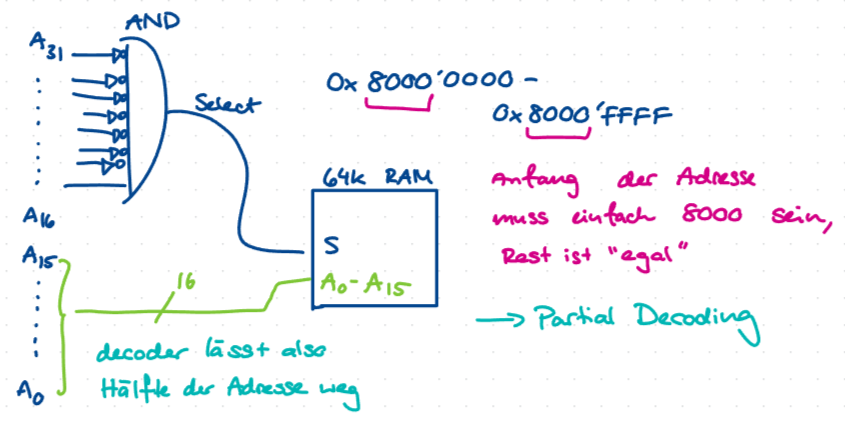
\includegraphics[width=\linewidth]{example_address_decoding2.png}
\end{example}

\subsubsection{Slow Slaves (Peripherals)}

\begin{definition}{Slow Slaves}\\
    Problem: Individual Slave Access times
    \begin{itemize}
        \item If slowest slave defines bus cycle time $\rightarrow$ reduced bus performance
        \item How can we get an individual bus cycle time for each slave?
    \end{itemize}   
\end{definition}

\begin{concept}{Solutions for slow slaves} two possibilities:
    \begin{itemize}
        \item \textbf{Individual Wait States} can be programmed at a bus interface unit \\
        Insert wait states to slow down the CPU to match the speed of the slowest peripheral (depending on the address of an access/bus cycle)\\
        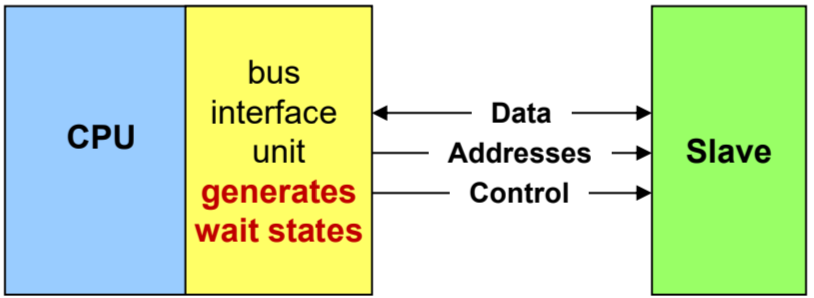
\includegraphics[width=\linewidth]{individual_wait_states.png}
        \item \textbf{Bus Mastering} Slave tells bus interface unit when it is ready \\
        Allow a peripheral to take control of the bus and perform its own accesses (e.g. DMA)\\
        Well suited for slaves with long or variable access times\\
        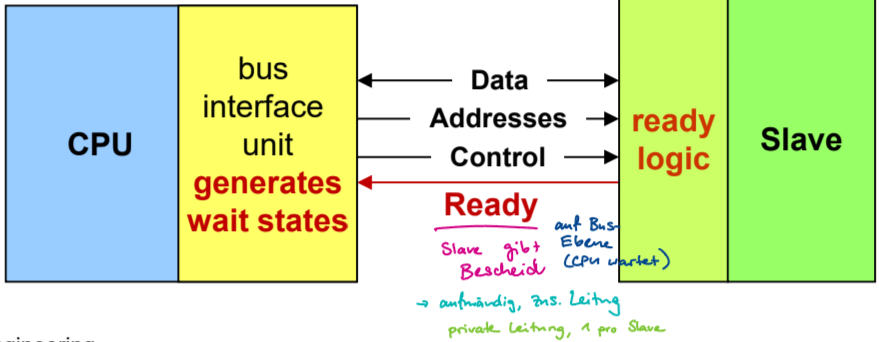
\includegraphics[width=\linewidth]{solution_for_slow_slaves.png}
    \end{itemize}
\end{concept}

\begin{KR}{Individual Wait States}\\
    Wait states are inserted to slow down the CPU to match the speed of the slowest peripheral (depending on the address of an access)

    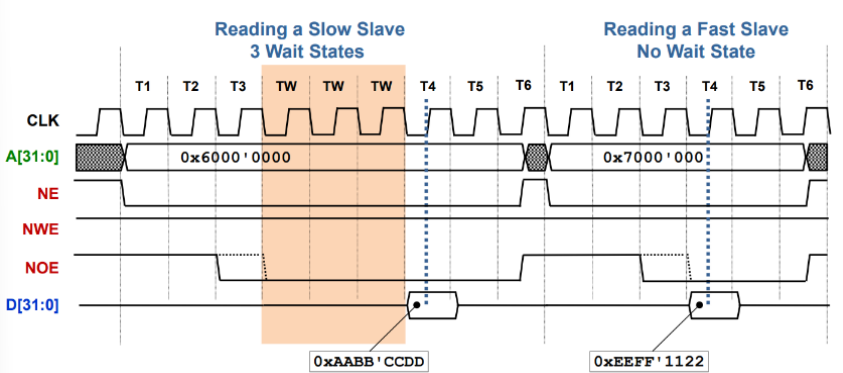
\includegraphics[width=\linewidth]{slow_slaves.png}    
\end{KR}



\subsubsection{Bus Hierarchies}

\begin{example2}{STM32 Microcontroller}\\
    with CPU, on-chip memory, and peripherals interconnected through the system bus(es)
    \begin{itemize}
        \item On-chip system bus: 32 data lines, 32 address lines and control signals
        \item Off-chip external bus: 16 data lines, 24 address lines and control signals
    \end{itemize}
    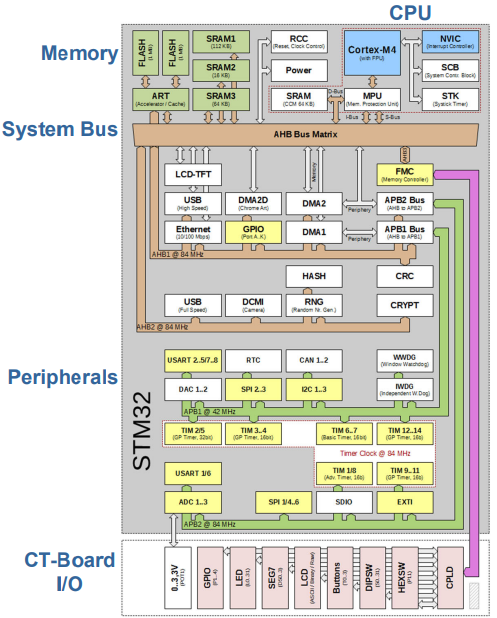
\includegraphics[width=0.9\linewidth]{stm32_example.png}

    A distributed system with parallel (simultaneous) processing of data in many peripherals. All under the supervision of the CPU.
\end{example2}

\begin{remark}
    Note: ARM calls their system buses AHB (ARM High-performance Bus) and APB (ARM
    Peripheral Bus). On complex chips, it is state-of-the-art to partition the system bus into
    multiple interconnected buses.
\end{remark}

\begin{example2}{CT Board with STM32 Microcontroller and Buses}\\
    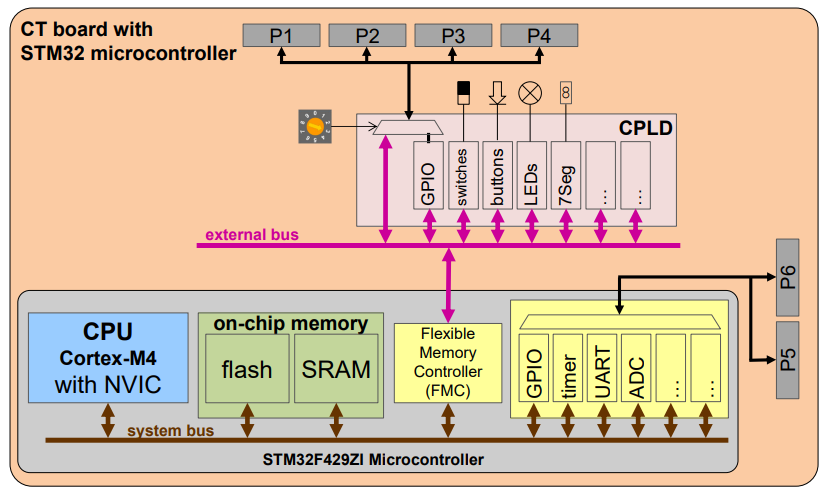
\includegraphics[width=\linewidth]{ctboard_with_stm32.png}\\
    Real-world Systems are partitioned into multiple buses.
\end{example2}


\subsubsection{Accessing Control Registers in C}

\begin{definition}{Accessing Control Registers in C}\\
    \textbf{Hardware View}
    \begin{itemize}
        \item Signals
        \item Timing
        \item Address decoding
        \item Wait states
        \item Control and status registers
    \end{itemize}
    \textbf{Software View}
    \begin{itemize}
        \item Accessing control and status registers in C
    \end{itemize}
\end{definition}

\begin{concept}{Problem}\\
    Compiler may remove statements that have no effect from the compiler's point of view\\
    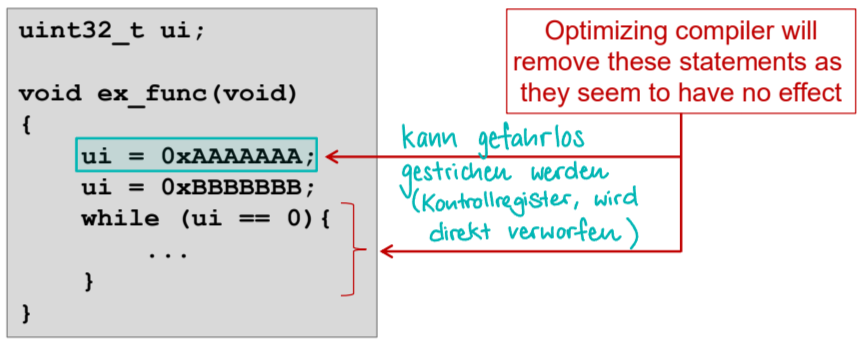
\includegraphics[width=\linewidth]{compiler_problems.png}
    \begin{itemize}
        \item Accesses to control registers (read/write) are memory accesses
        \item If writing has a side effect on the hardware and/or if reading may result in a different value than was set before in the code,
        the program will not behave as intended/expected
    \end{itemize}
\end{concept}

\begin{theorem}{Solution}\\
    \begin{itemize}
        \item Use the \texttt{volatile} keyword/qualifier in C to prevent the compiler from removing statements that have no effect from the compiler's point of view\\
        $\rightarrow$ prohibit compiler optimizations on the variable\\
        \item The compiler will not optimize away accesses to a variable declared as volatile
        \item The compiler will not reorder accesses to a variable declared as volatile
    \end{itemize}
    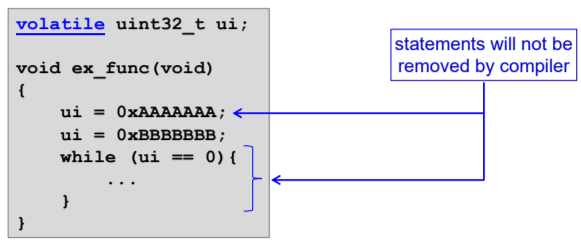
\includegraphics[width=\linewidth]{volatile_keyword.png}
    \begin{itemize}
        \item Tell compiler that the variable may change at any time, outside the control of the compiler (e.g. by hardware or interrupt handler)
        \item The compiler cannot make any assumptions about the value of the variable\\
        needs to execute all read/write accesses as programmed\\
        prevents compiler optimizations
    \end{itemize}
\end{theorem}

\begin{corollary}{Access through Pointers} e.g. writing to and reading from CT Board I/O\\
    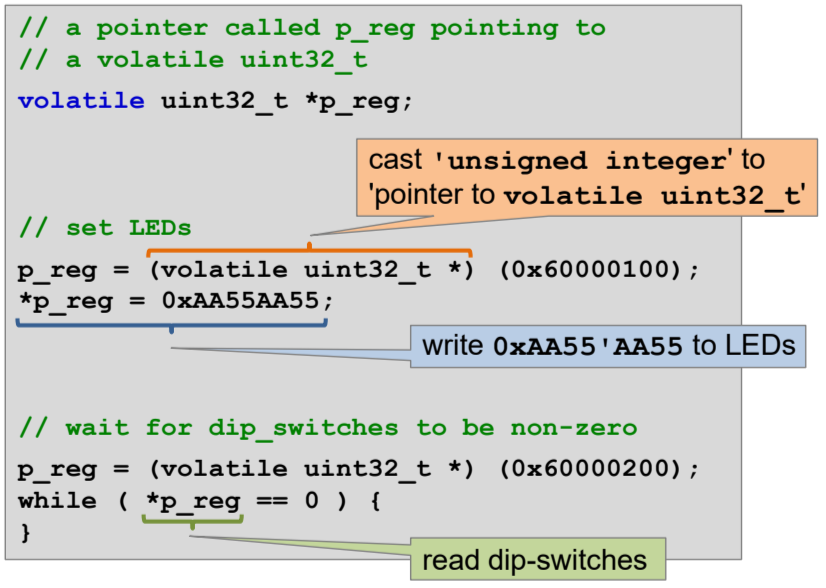
\includegraphics[width=\linewidth]{access_through_pointers1.png}\\
    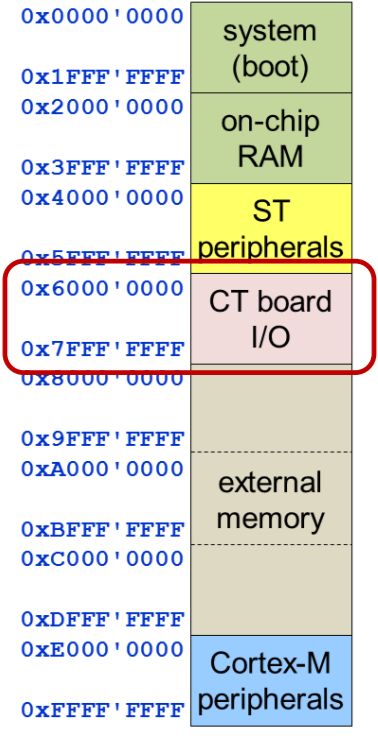
\includegraphics[width=\linewidth]{access_through_pointers2.png}
\end{corollary}

\begin{examplecode}{Using Preprocessor Macros} $\rightarrow$ \#define
\begin{lstlisting}[language=C, style=basesmol]
#define LED31_0_REG (*((volatile uint32_t *) 0x60000100))

#define BUTTON_REG (*((volatile uint32_t *) 0x60000210))

//Write LED register to 0xBBCC'DDEE
LED31_0_REG = 0xBBCCDDEE;
//Read Button register to aux_var
aux_var = BUTTON_REG;
\end{lstlisting}
    \vspace{2mm}
    \texttt{(\textcolor{darkturquoise}{*}(\textcolor{pink}{(volatile\ uint32\_t *)} 0x60000100))}\\
    $\rightarrow$ \textcolor{darkturquoise}{dereference} the pointer to the register address\\
    $\rightarrow$ \textcolor{pink}{cast} the address to a pointer to a 32-bit register
\end{examplecode}





\subsection{Conclusions}
\begin{KR}{Conclusions}
    Microcontrollers $\rightarrow$ Embedded Systems
- Low cost, real time, low power, extreme environments System Bus
- Address, data and control lines
- Synchronous or asynchronous
- CPU (master) reads from or writes to slave
- Timing sequences
- Wait states

Address Decoding
- Who is the CPU talking to?
- Full vs. partial address decoding

Accessing Control Registers in C
- Qualifier volatile
- Use of pointers for memory accesses
\end{KR}

\begin{remark}
    Learning Objectives:\\
    At the end of this lesson, you will be able
- to enumerate the signal groups of a system bus
- to distinguish between 'synchronous' and 'asynchronous' bus timing
- to know what the term 'tri-state' means
- to interpret simple bus timing diagrams
- to describe the concept of a bus and how data is transferred on a bus
- to describe the function and purpose of control and status registers
- to explain the terms 'full address decoding' and 'partial address decoding'
- to access control registers from C
- to explain the meaning of the qualifier 'volatile' in C
- to analyze address decoding logic and to derive the applicable addresses or address ranges
- to derive an address decoding logic for a given address (range)
- to explain the function of wait states
\end{remark}















